
\hypertarget{working_toolsbar}{}
\section{Tools bar}
\index{toolsbar}

\begin{figure}[h!]
  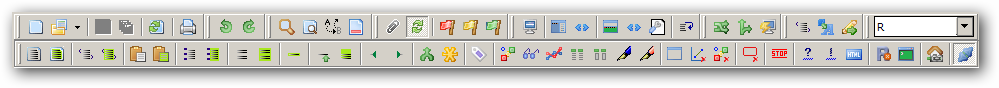
\includegraphics[scale=0.35]{./res/toolsbar.png}\\
  \caption{Tools bar.}
  \label{fig:toolsbar}
\end{figure}

\begin{table}[h!]
  \begin{footnotesize}
    \begin{tabularx}{\textwidth}{>{\hsize=0.3\hsize}X>{\hsize=0.7\hsize}X}\\
      \hline
      \textbf{Category} & \textbf{Description} \\
      \hline
      File & New, open, save, save all, reload and print \\
      Edit & Undo and redo \\
      Filter & Create a new file with all occurrences of typed sequence of characters \\
      Macro & Record and play \\
      Misc & On top, focus control and block marks \\
      Processing & Conversion, compilation and viewer \\
      \RR{} & Lots of options to send and control \RR{} \\
      Search & Current file, in files, replace and go to line \\
      Syntax & Drop down list of all syntaxes available \\
      Spell & Drop down list of installed dictionaries and a bottom to start the speller \\
      View & Organize screen, Tools (show/hide), Tools (size), Rterm (show/hide, Rterm (size), options to \textit{IO} and \textit{Log} and word wrap \\
      \hline
    \end{tabularx}
  \end{footnotesize}
  \caption{Tools bar.}
  \label{tab:toolsbar}
\end{table}

Unlike most applications of this category, this interface
(Figure \ref{fig:toolsbar})
was designed to be
as small and simple as possible. In other words, the full access to all
resources of Tinn-R are available at the main menu and associated shortcuts
(it takes time to learn all and most are user configurable).

Two groups are available: main and \RR{} tool bar.

The main toolbar interface is categorized
(Table \ref{tab:toolsbar})
and contains the most common tasks:

The \RR{} toolbar has two basic divisions: Send (left side, finishing in the
\textit{Set work directory buttom}) and Control (right side, starting
in the \textit{List all objects buttom}).


\hypertarget{working_toolsbar_showhide}{}
\subsection{Show/Hide}
\index{toolsbar!showhide}

\begin{figure}[h!]
  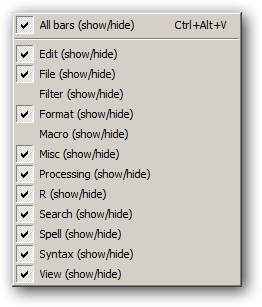
\includegraphics[scale=0.35]{./res/toolsbar_pmenu.png}\\
  \caption{Tools bar menu.}
  \label{fig:toolsbar_pmenu}
\end{figure}

The Tools bar has its own pop-up
(Figure \ref{fig:toolsbar_pmenu})
menu enabling the user to choose what
resources will be visible (show/hide). To see the pop-up menu, press the
right mouse buttom inside any place of the main tool bar.


\hypertarget{working_toolsbar_disposition}{}
\subsection{Disposition}
\index{toolsbar!disposition}

The interface also allows drag and drop. In other words, you can organize
the order of the individual tool bar inside of the main container.

It is better to do that with the main interface not maximized to avoid
screen flicker (a small nuance related to some version of the Windows
and Borland engine).
